\begin{figure*}[t]
  \centering
  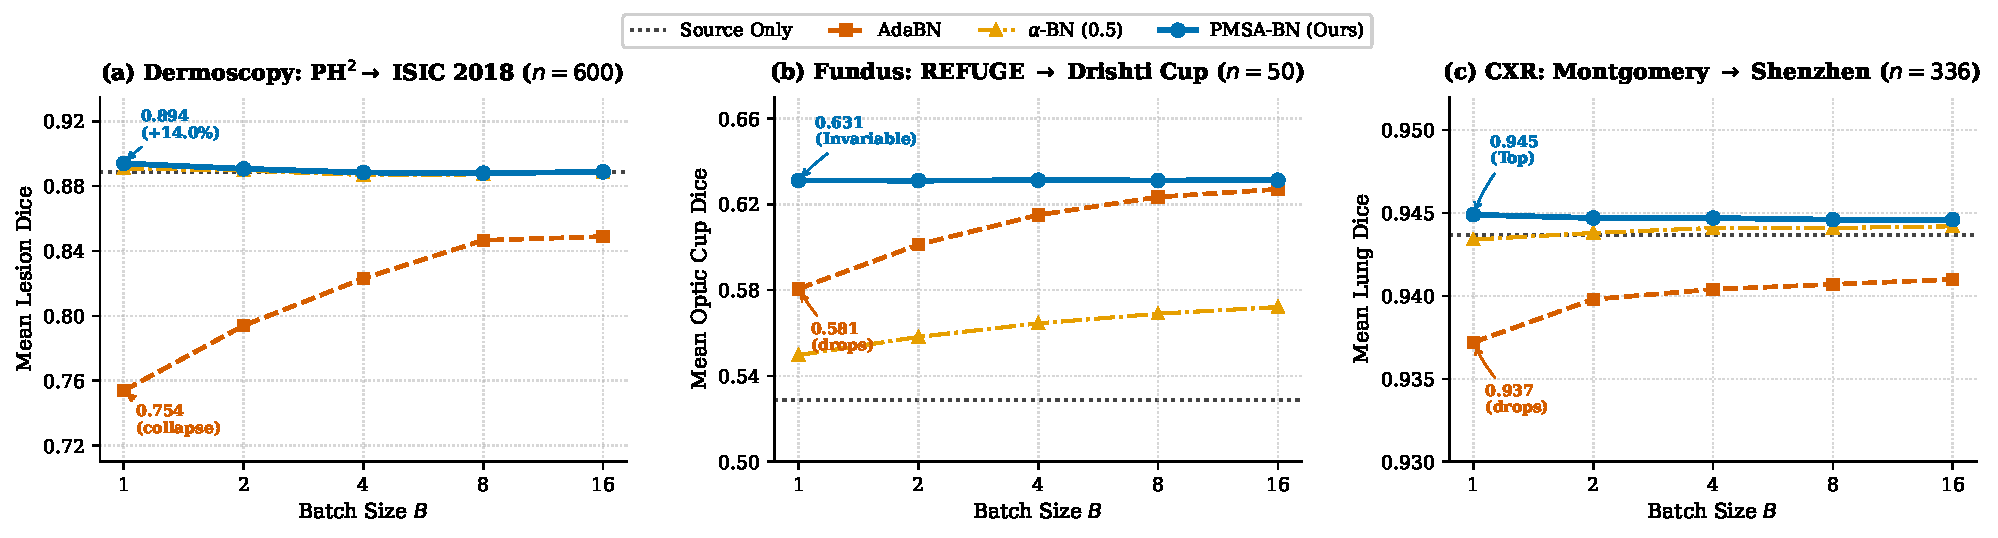
\includegraphics[width=0.98\linewidth]{fig1_batch_size.pdf}
  \caption{Test Dice versus adaptation batch size $B \in \{1, 2, 4, 8, 16\}$ across the three modalities evaluated in our ablation study: (a) Dermoscopy (PH$^2 \to$ ISIC 2018), (b) Endoscopy (Kvasir $\to$ ClinicDB), and (c) Retinal Fundus (REFUGE $\to$ Drishti-GS). Standard AdaBN relies on multi-sample statistics and severely degrades at $B=1$ (dropping by up to $-14.0\%$ on dermoscopy and $-6.4\%$ on polyps). In contrast, PMSA-BN achieves immediate top performance at $B=1$ across all three modalities and maintains near-perfect batch-size invariance.}
  \label{fig:batch_size}
\end{figure*}
